\section{Magnetische Felder}

\vspace{1\baselineskip}

Es gilt: $I = \frac{dq}{dt} = \frac{dl}{dt} \frac{dq}{dx} = v \cdot \lambda$
mit $\lambda$ der \fat{Linienladungsdichte}.

\vspace{1\baselineskip}

\fat{Lorentz-Kraft}: Kraft, welche auf bewegte Teilchen in einem Magnetfeld wirkt:
\begin{align*}
    d \vec{F}_L = I (d \vec{l} \times \vec{B}(\vec{r}))
    \quad \text{oder allgemeiner} \quad
    \vec{F} = q \klammer{\vec{E} + \vec{v} \times \vec{B}}
\end{align*}
Mit $I$ Strom, $\vec{B}$ Magnetfeld, $q$ (positive) Ladung des Teilchens,
$E$ elektrisches Feld, $d \vec{r}$ Leiterelement.
\begin{center}
    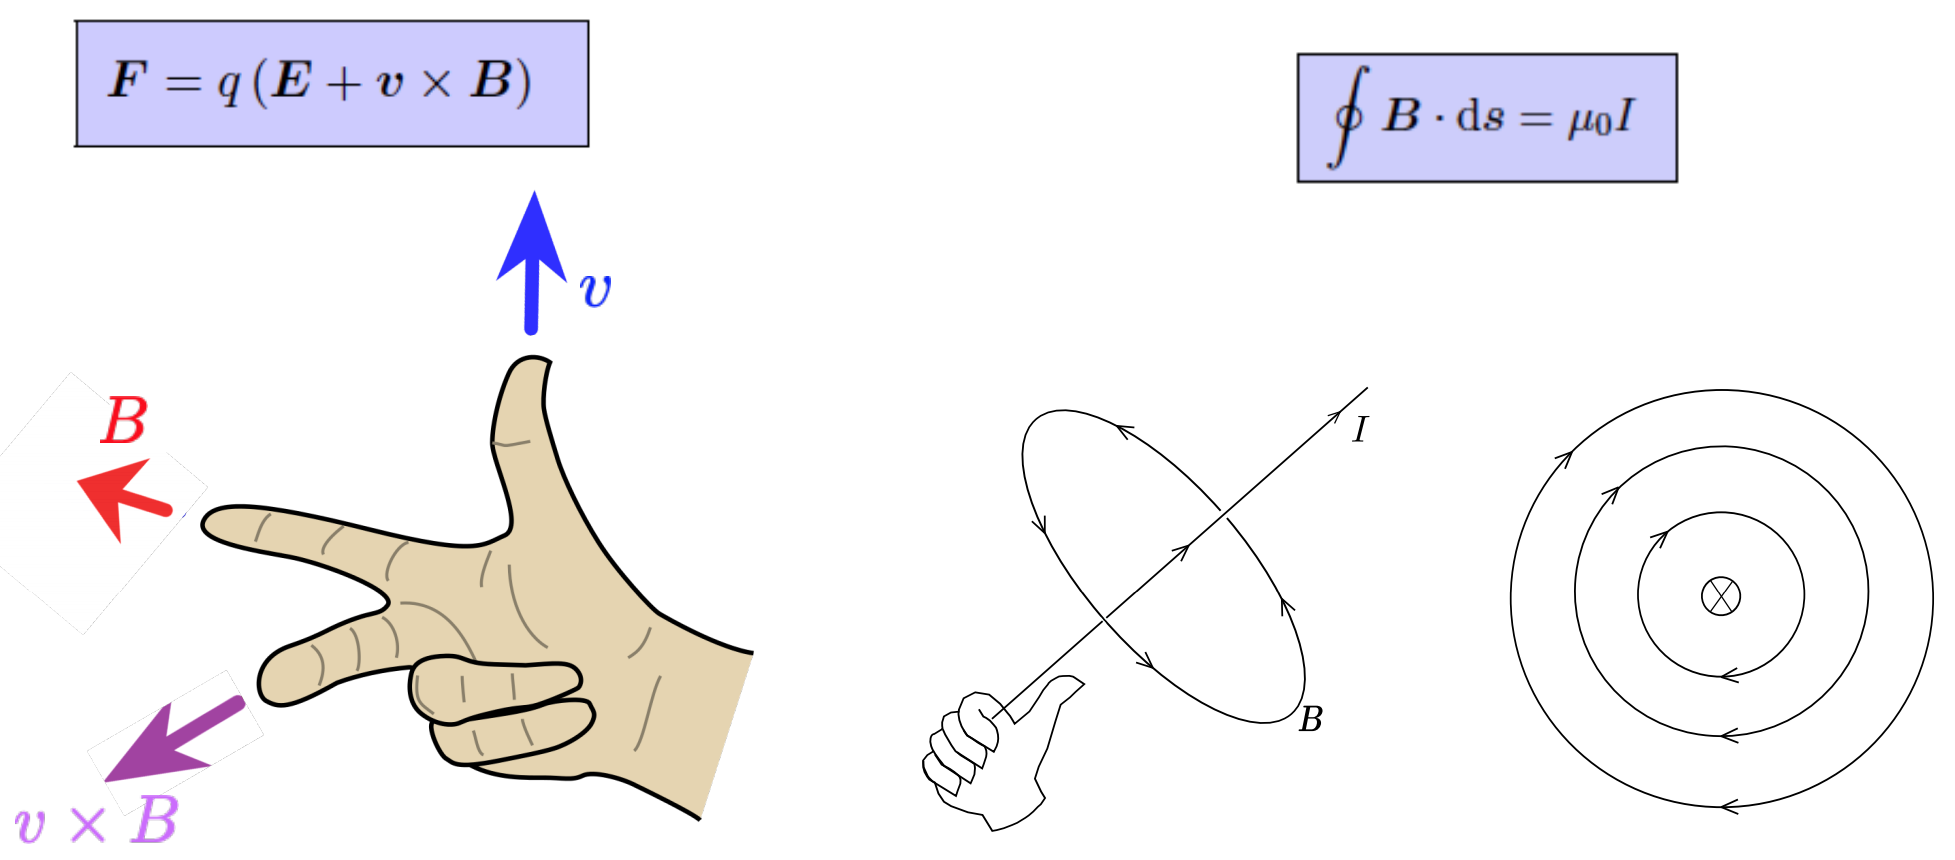
\includegraphics[width=0.4\textwidth]{Figures/3FingerRegel.png}
\end{center}

\vspace{1\baselineskip}

\begin{tcolorbox}
    Das \fat{Ampère'sche Gesetz} wird benutzt, wenn wir unendlich ausgedehnte Leiter haben,
    wie zB einen unendlich langen Draht. Die Formel lautet: 

    \begin{equation*}
        \oint_S \vec{B} \cdot d \vec{s} = \mu_0 I_{\mathrm{eing.}}
        \quad \quad \text{  oder  } \quad \quad
        \vec{\nabla} \times \vec{B} = \munull 
    \end{equation*}

    \subsubsection*{Vorgehen}

    \begin{enumerate}
        \item Skizze zeichnen + Koordinaten wählen
        \item Schleife einzeichnen
        \item Erste Formel für Ampère'sches Gesetz benutzen
        \item Auflösen
    \end{enumerate}
\end{tcolorbox}

\vspace{1\baselineskip}

\fat{Eindeutigkeitssatz}: Für eine gegebene Konfiguration von Strömen $\vec{J}(\vec{r})$
existiert ein eindeutiges Magnetfeld $\vec{B}(\vec{r})$.

\vspace{1\baselineskip}

\fat{Das Vektorpotential} ist definiert als:
\begin{align*}
    \vec{A}(\vec{r}) = \frac{\munull}{4 \pi} \int_{\R^3} \frac{\vec{J}(\vec{r'})}{\abs{\vec{r}-\vec{r'}}} dx' dy' dz'
    \quad \quad \Leftrightarrow \quad \quad \Delta \vec{A} = - \munull \vec{J}
\end{align*}

\vspace{1\baselineskip}

\fat{Das Biot-Savart'sche Gesetz}

\begin{tcolorbox}
    Die Formel von Biot-Savart lautet wie folgt: 
    \begin{equation*}
        d\Vec{B}(\Vec{r}) = \frac{\mu_0}{4 \pi}I d\Vec{l} \times \frac{\Vec{r}- \Vec{r}'}{|\Vec{r}- \Vec{r}'|^3}
        = \frac{\mu_0 I}{4 \pi r^2} (d \vec{l} \times \hat{r})
        = \frac{\mu_0}{4 \pi r^2} (\vec{J} \times \hat{r}) dV
    \end{equation*}
    \begin{align*}
        \vec{B} = \frac{\munull q}{4 \pi r^2} (\vec{v} \times \hat{r})
    \end{align*}
    \begin{itemize}
        \item \textbf{Leiterelement $d\vec{l}$:} \\
        Wir wählen uns auf jedem Leiter ein infinitesimales Leiterelement. Dies beschreiben wir
        dann im gewählten Koordinatensystem. Es beschreibt also einen kleinen Ausschnitt auf dem
        Leiter. Später wird dann über dieses Element integriert.
        \item \textbf{Position des Leiterelements $ \vec{r}'$:} \\
        Der gestrichene Ortsvektor beschreibt die Position des Leiterelements.
        \item \textbf{Position des Betrachtungspunkts P $\vec{r}$:}
        Um das magnetische Feld letzten Ende zu berechnen, betrachten wir einen bestimmten Punkt in
        allgemeinen Koordinaten, dh. wir können ihn überall wählen, jedoch ist manchmal ein
        bestimmter Punkt gefragt und dann vereinfacht sich die Formel.
    \end{itemize}

    \paragraph{Vorgehen:}
    \begin{enumerate}
        \item $d\vec{l}$ definieren
        \item Position von P bestimmen ($\vec{r}$)
        \item Position von $d\vec{l}$ bestimmen ($\vec{r}'$)
        \item Erste Formel von Biot-Savart verwenden
    \end{enumerate}
\end{tcolorbox}

\vspace{1\baselineskip}

\fat{Energiedichte}
\begin{itemize}
    \item des Magnetfeldes: $u_B = \frac{B^2}{2 \munull}$
    \item des elektrischen Feldes: $u_E = \frac{\epsilonnull E^2}{2}$
\end{itemize}

\vspace{1\baselineskip}

\fat{Hall-Effekt}

In Magnetfeldern wirkt auf bewegte Ladungen eine zu ihrer Bewegungsrichtung senkrecht wirkende
Kraft. In einem stromdurchflossenen Leiter schiebt diese Kraft die Ladungsträger auf eine Seite
des Leiters, und es kommt zu einer Ladungstrennung. Zwischen der oberen und der unteren Seite
des Ladungsträgers entsteht dann eine Spannungsdifferenz, die sogenannte \fat{Hall-Spannung}
\begin{align*}
    U_H = E_H b = v_d B b
\end{align*}

\vspace{1\baselineskip}

\fat{Magnetischer Dipolmoment}

Das magnetische Moment einer Leiterschleife ist gegeben durch:
\begin{align*}
    \vec{\mu} = n I \vec{A}
\end{align*}
wobei $n$ die Anzahl Windungen der Leiterschleife ist. Auf eine Leiterschleife wirkt nun ein
Drehmoment, welches gegeben ist durch
\begin{align*}
    \vec{M} = \vec{\mu} \times \vec{B}
\end{align*}

\vspace{1\baselineskip}

\fat{Relativistische Transformationen}

Wir betrachten einen unendlich ausgedehnten Plattenkondensator parallel zur $xz$-Ebene,
welche sich im Laborsystem $K$ mit der geschwindigkeit $v_0$ in $x$-Richtung bewegt.
Sei $K'$ ein Inertialsystem das sich mit $v$ relativ zu $K$ in $x$-Richtung bewegt
($\beta = \frac{v}{c}$).
\begin{align*}
    E'_{\parallel} &= E_{\parallel}
    \quad \quad \quad \quad
    \vec{E'}_{\perp} = \gamma \klammer{\vec{E}_{\perp} + c \vec{\beta} \times \vec{B}_{\perp}}
    \\
    B'_{\parallel} &= B_{\parallel}
    \quad \quad \quad \quad
    \vec{B'}_{\perp} = \gamma \klammer{\vec{B}_{\perp} - \frac{1}{c} \vec{\beta} \times \vec{E}_{\perp}}
\end{align*}
Im Spezialfall $\vec{B} = 0$:
\begin{align*}
    E'_{\parallel} &= E_{\parallel}
    \quad \quad \quad \quad
    \vec{E'}_{\perp} = \gamma \vec{E}_{\perp}
    \\
    B'_{\parallel} &= 0
    \quad \quad \quad \quad
    \vec{B'}_{\perp} = - \gamma \frac{\vec{\beta}}{c} \times \vec{E}_{\perp}
\end{align*}
Wegen $\vec{\beta} \times \vec{E}_{\parallel} = 0$ folgt:
\begin{align*}
    \vec{B'} = - \frac{\vec{\beta}}{c} \times \vec{E'}
\end{align*}
